\documentclass[landscape]{article}
\usepackage[dvipsnames]{xcolor}
\usepackage{tikz}

\usetikzlibrary{patterns,snakes}
\usepackage{stackengine}

\begin{document}


\begin{center}
  \hspace{-3.0in}
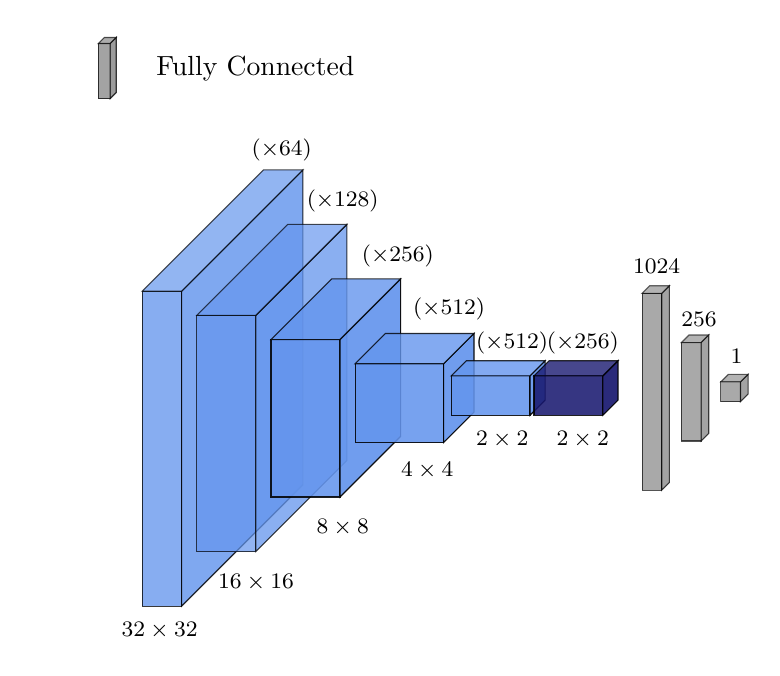
\begin{tikzpicture}[scale=0.5]
  %%%%%%%%%%%%%%%%%%%%%%%%%%%%%%%%%%%%%%%%%%%%%%%%%%%%%%%%%%%%%%%%%%%%%%%%%%%%%%%%%%%%%%%%%%%%%%%%%%%%%%%%%%%%%%%%%%%%%%%%%%
  %%%  PARAMETERS:
  %%%%%%%%%%%%%%%%%%%%%%%%%%%%%%%%%%%%%%%%%%%%%%%%%%%%%%%%%%%%%%%%%%%%%%%%%%%%%%%%%%%%%%%%%%%%%%%%%%%%%%%%%%%%%%%%%%%%%%%%%%

  
  %%% COLOR PALLETE %%%
  \def\colora{CornflowerBlue}
  \def\colorb{Gray}
  \def\colorf{MidnightBlue}
  
  %%% CENTER X-Y COORDINATES
  \def\cx{0}
  \def\cy{0}

  %%% FRONT/SIDE/TOP OPACITIES
  \def\fopac{0.875}
  \def\sopac{0.925}
  \def\topac{0.8}

  \def\fopacb{0.675}
  \def\sopacb{0.725}
  \def\topacb{0.6}


  %%%%%%%%%%%%%%%%%%%%%%%%%%%%
  %%% LEGEND
  %%%%%%%%%%%%%%%%%%%%%%%%%%%%

  %%% CENTER X-Y COORDINATES
  \def\cx{0}
  \def\cy{0}

  \node at (0,8) {
    \setlength\tabcolsep{2pt}
    \begin{tabular}{cc}
      \def\depth{0.15}
      \def\res{0.35}
      \def\resalt{0.1}
      \def\initd{0}
      \def\fcolor{\colorb}
      \tikz{\draw[fill=\fcolor,opacity=0.725] (\initd,\cx-\res,\cy+\resalt) -- ++(\depth,0,0) -- ++(0,2*\res,0) -- ++(-\depth,0,0) -- cycle;
      \draw[fill=\fcolor,opacity=0.775] (\initd+\depth,\cx-\res,\cy+\resalt) -- ++(0,0,-2*\resalt) -- ++(0,2*\res,0) -- ++(0,0,2*\resalt) -- cycle;
      \draw[fill=\fcolor,opacity=0.65] (\initd,\cx+\res,\cy+\resalt) -- ++(\depth,0,0) -- ++(0,0,-2*\resalt) -- ++(-\depth,0,0) -- cycle;}
      & \raisebox{0.12in}{ \hspace{0.05in} Fully Connected} \hspace{0.0in} 
      %%%%%%%%%%%%%%%%%%%%%%%%%%%%%%%%%%%%%%%%%%%%%%%%%%%%%%%%%%%%%%%%%%%%%%%%%%%
    \end{tabular}
  };
  
  %%%%%%%%%%%%%%%%%%%%%%%%%%%%%%%%%%%%%%%%%%%%%%%%%%%%%%%%%%%%%%%%%%%%%%%%%%%%%%%%%%%%%%%%%%%%%%%%%%%%%%%%%%%%%%%%%%%%%%%%%%
  %%%   LAYERS
  %%%%%%%%%%%%%%%%%%%%%%%%%%%%%%%%%%%%%%%%%%%%%%%%%%%%%%%%%%%%%%%%%%%%%%%%%%%%%%%%%%%%%%%%%%%%%%%%%%%%%%%%%%%%%%%%%%%%%%%%%%
  \def\dfactor{0.25}
  \def\initd{0}
  \def\depth{1}
  \def\res{4}
  \def\fcolor{\colora}
  %% FRONT
  \draw[fill=\fcolor,opacity=0.775] (\initd,\cx-\res,\cy+\res) -- ++(\depth,0,0) -- ++(0,2*\res,0) -- ++(-\depth,0,0) -- cycle;
  %% SIDE
  \draw[fill=\fcolor,opacity=0.825] (\initd+\depth,\cx-\res,\cy+\res) -- ++(0,0,-2*\res) -- ++(0,2*\res,0) -- ++(0,0,2*\res) -- cycle;
  %% TOP
  \draw[fill=\fcolor,opacity=0.7] (\initd,\cx+\res,\cy+\res) -- ++(\depth,0,0) -- ++(0,0,-2*\res) -- ++(-\depth,0,0) -- cycle;
  \node at (2,6.05) {\footnotesize$(\times 64)$};
  \node at (2-3.1,-6.05-0.1) {\footnotesize$32\times32$};
  %%%%%%%%%%%%%%%%%%%%%%%%%%%%%%%%%%%%%%%%%%%%%%%%%%%%%%%%%%%%%%%%%%%%%%%%%%%%%%%%%%%%%%%%%%%%%%%%%%%%%%%%%%%%%%%%%%%%%%%%%%
  \def\initd{1}
  \def\depth{1.5}
  \def\res{3}
  \def\fcolor{\colora}
  \draw[fill=\fcolor,opacity=0.705] (\initd,\cx-\res,\cy+\res) -- ++(\depth,0,0) -- ++(0,2*\res,0) -- ++(-\depth,0,0) -- cycle;
  \draw[fill=\fcolor,opacity=0.755] (\initd+\depth,\cx-\res,\cy+\res) -- ++(0,0,-2*\res) -- ++(0,2*\res,0) -- ++(0,0,2*\res) -- cycle;
  \draw[fill=\fcolor,opacity=0.685] (\initd,\cx+\res,\cy+\res) -- ++(\depth,0,0) -- ++(0,0,-2*\res) -- ++(-\depth,0,0) -- cycle;
  \node at (3.55,4.75) {\footnotesize$(\times 128)$};
  \node at (3.75-2.4,-4.75-0.2) {\footnotesize$16\times16$};
  %%%%%%%%%%%%%%%%%%%%%%%%%%%%%%%%%%%%%%%%%%%%%%%%%%%%%%%%%%%%%%%%%%%%%%%%%%%%%%%%%%%%%%%%%%%%%%%%%%%%%%%%%%%%%%%%%%%%%%%%%%
  \def\initd{2.5}
  \def\depth{1.75}
  \def\res{2}
  \def\fcolor{\colora}
  \draw[fill=\fcolor,opacity=\fopac] (\initd,\cx-\res,\cy+\res) -- ++(\depth,0,0) -- ++(0,2*\res,0) -- ++(-\depth,0,0) -- cycle;
  \draw[fill=\fcolor,opacity=\sopac] (\initd+\depth,\cx-\res,\cy+\res) -- ++(0,0,-2*\res) -- ++(0,2*\res,0) -- ++(0,0,2*\res) -- cycle;
  \draw[fill=\fcolor,opacity=\topac] (\initd,\cx+\res,\cy+\res) -- ++(\depth,0,0) -- ++(0,0,-2*\res) -- ++(-\depth,0,0) -- cycle;
  \node at (4.95,3.35) {\footnotesize$(\times 256)$};
  \node at (4.75-1.2,-3.5-0.05) {\footnotesize$8\times8$};


  %%%%%%%%%%%%%%%%%%%%%%%%%%%%%%%%%%%%%%%%%%%%%%%%%%%%%%%%%%%%%%%%%%%%%%%%%%%%%%%%%%%%%%%%%%%%%%%%%%%%%%%%%%%%%%%%%%%%%%%%%%



  
  %%%%%%%%%%%%%%%%%%%%%%%%%%%%%%%%%%%%%%%%%%%%%%%%%%%%%%%%%%%%%%%%%%%%%%%%%%%%%%%%%%%%%%%%%%%%%%%%%%%%%%%%%%%%%%%%%%%%%%%%%%
  \def\initd{4.25}
  \def\depth{2.25}
  \def\res{1}
  \def\fcolor{\colora}
  \draw[fill=\fcolor,opacity=\fopac] (\initd,\cx-\res,\cy+\res) -- ++(\depth,0,0) -- ++(0,2*\res,0) -- ++(-\depth,0,0) -- cycle;
  \draw[fill=\fcolor,opacity=\sopac] (\initd+\depth,\cx-\res,\cy+\res) -- ++(0,0,-2*\res) -- ++(0,2*\res,0) -- ++(0,0,2*\res) -- cycle;
  \draw[fill=\fcolor,opacity=\topac] (\initd,\cx+\res,\cy+\res) -- ++(\depth,0,0) -- ++(0,0,-2*\res) -- ++(-\depth,0,0) -- cycle;
  \node at (6.25,2.0) {\footnotesize$(\times 512)$};
  \node at (6.45-0.75,-2.0-0.1) {\footnotesize$4\times4$};
  %%%%%%%%%%%%%%%%%%%%%%%%%%%%%%%%%%%%%%%%%%%%%%%%%%%%%%%%%%%%%%%%%%%%%%%%%%%%%%%%%%%%%%%%%%%%%%%%%%%%%%%%%%%%%%%%%%%%%%%%%%
  \def\initd{6.5}
  \def\depth{2.0}
  \def\res{0.5}
  \def\fcolor{\colora}
  \draw[fill=\fcolor,opacity=\fopac] (\initd,\cx-\res,\cy+\res) -- ++(\depth,0,0) -- ++(0,2*\res,0) -- ++(-\depth,0,0) -- cycle;
  \draw[fill=\fcolor,opacity=\sopac] (\initd+\depth,\cx-\res,\cy+\res) -- ++(0,0,-2*\res) -- ++(0,2*\res,0) -- ++(0,0,2*\res) -- cycle;
  \draw[fill=\fcolor,opacity=\topac] (\initd,\cx+\res,\cy+\res) -- ++(\depth,0,0) -- ++(0,0,-2*\res) -- ++(-\depth,0,0) -- cycle;
  \node at (7.85,1.15) {\footnotesize$(\times 512)$};
  \node at (7.85-0.25,-1.15-0.15) {\footnotesize$2\times2$};
  %%%%%%%%%%%%%%%%%%%%%%%%%%%%%%%%%%%%%%%%%%%%%%%%%%%%%%%%%%%%%%%%%%%%%%%%%%%%%%%%%%%%%%%%%%%%%%%%%%%%%%%%%%%%%%%%%%%%%%%%%%
  
  %%%%%%%%%%%%%%%%%%%%%%%%%%%%%%%%%%%%%%%%%%%%%%%%%%%%%%%%%%%%%%%%%%%%%%%%%%%%%%%%%%%%%%%%%%%%%%%%%%%%%%%%%%%%%%%%%%%%%%%%%%
  %%%    CENTER / NOISE FILTER
  %%%%%%%%%%%%%%%%%%%%%%%%%%%%%%%%%%%%%%%%%%%%%%%%%%%%%%%%%%%%%%%%%%%%%%%%%%%%%%%%%%%%%%%%%%%%%%%%%%%%%%%%%%%%%%%%%%%%%%%%%%
  \def\initd{8.6}
  \def\depth{1.75}
  \def\centerdepth{9.0+2.0}
  \def\res{0.5}
  \def\fcolor{\colorf}
  \draw[fill=\fcolor,opacity=\fopac] (\initd,\cx-\res,\cy+\res) -- ++(\depth,0,0) -- ++(0,2*\res,0) -- ++(-\depth,0,0) -- cycle;
  \draw[fill=\fcolor,opacity=\sopac] (\initd+\depth,\cx-\res,\cy+\res) -- ++(0,0,-2*\res) -- ++(0,2*\res,0) -- ++(0,0,2*\res) -- cycle;
  \draw[fill=\fcolor,opacity=\topac] (\initd,\cx+\res,\cy+\res) -- ++(\depth,0,0) -- ++(0,0,-2*\res) -- ++(-\depth,0,0) -- cycle;
  \node at (9.65,1.15-0.0) {\footnotesize$(\times 256)$};
  \node at (9.65,-1.15-0.15) {\footnotesize$2\times2$};
  %%%%%%%%%%%%%%%%%%%%%%%%%%%%%%%%%%%%%%%%%%%%%%%%%%%%%%%%%%%%%%%%%%%%%%%%%%%%%%%%%%%%%%%%%%%%%%%%%%%%%%%%%%%%%%%%%%%%%%%%%%


  
  %%%%%%%%%%%%%%%%%%%%%%%%%%%%%%%%%%%%%%%%%%%%%%%%%%%%%%%%%%%%%%%%%%%%%%%%%%%%%%%%%%%%%%%%%%%%%%%%%%%%%%%%%%%%%%%%%%%%%%%%%%
  %%%    FULLY CONNECTED
  %%%%%%%%%%%%%%%%%%%%%%%%%%%%%%%%%%%%%%%%%%%%%%%%%%%%%%%%%%%%%%%%%%%%%%%%%%%%%%%%%%%%%%%%%%%%%%%%%%%%%%%%%%%%%%%%%%%%%%%%%%
  \def\initd{\centerdepth+0.25}
  \def\depth{0.5}
  \def\resx{2.5}
  \def\resy{0.25}
  \def\fcolor{\colorb}
  \draw[fill=\fcolor,opacity=\fopacb] (\initd,\cx-\resx,\cy+\resy) -- ++(\depth,0,0) -- ++(0,2*\resx,0) -- ++(-\depth,0,0) -- cycle;
  \draw[fill=\fcolor,opacity=\sopacb] (\initd+\depth,\cx-\resx,\cy+\resy) -- ++(0,0,-2*\resy) -- ++(0,2*\resx,0) -- ++(0,0,2*\resy) -- cycle;
  \draw[fill=\fcolor,opacity=\topacb] (\initd,\cx+\resx,\cy+\resy) -- ++(\depth,0,0) -- ++(0,0,-2*\resy) -- ++(-\depth,0,0) -- cycle;
  \node at (\centerdepth+2.275-1.75,3.1) {\footnotesize$1024$};
  %\node at (8.35,1.15) {\footnotesize$(\times 512)$};
  %\node at (8.35-0.25,-1.15-0.15) {\footnotesize$2\times2$};
  %%%%%%%%%%%%%%%%%%%%%%%%%%%%%%%%%%%%%%%%%%%%%%%%%%%%%%%%%%%%%%%%%%%%%%%%%%%%%%%%%%%%%%%%%%%%%%%%%%%%%%%%%%%%%%%%%%%%%%%%%%
  \def\initd{\centerdepth+1.25}
  \def\depth{0.5}
  \def\resx{1.25}
  \def\resy{0.25}
  \def\fcolor{\colorb}
  \draw[fill=\fcolor,opacity=\fopacb] (\initd,\cx-\resx,\cy+\resy) -- ++(\depth,0,0) -- ++(0,2*\resx,0) -- ++(-\depth,0,0) -- cycle;
  \draw[fill=\fcolor,opacity=\sopacb] (\initd+\depth,\cx-\resx,\cy+\resy) -- ++(0,0,-2*\resy) -- ++(0,2*\resx,0) -- ++(0,0,2*\resy) -- cycle;
  \draw[fill=\fcolor,opacity=\topacb] (\initd,\cx+\resx,\cy+\resy) -- ++(\depth,0,0) -- ++(0,0,-2*\resy) -- ++(-\depth,0,0) -- cycle;
  \node at (\centerdepth+3.35-1.75,1.75) {\footnotesize$256$};
  %\node at (8.35,1.15) {\footnotesize$(\times 512)$};
  %\node at (8.35-0.25,-1.15-0.15) {\footnotesize$2\times2$};
  %%%%%%%%%%%%%%%%%%%%%%%%%%%%%%%%%%%%%%%%%%%%%%%%%%%%%%%%%%%%%%%%%%%%%%%%%%%%%%%%%%%%%%%%%%%%%%%%%%%%%%%%%%%%%%%%%%%%%%%%%%
  \def\initd{\centerdepth+2.25}
  \def\depth{0.5}
  \def\resx{0.25}
  \def\resy{0.25}
  \def\fcolor{\colorb}
  \draw[fill=\fcolor,opacity=\fopacb] (\initd,\cx-\resx,\cy+\resy) -- ++(\depth,0,0) -- ++(0,2*\resx,0) -- ++(-\depth,0,0) -- cycle;
  \draw[fill=\fcolor,opacity=\sopacb] (\initd+\depth,\cx-\resx,\cy+\resy) -- ++(0,0,-2*\resy) -- ++(0,2*\resx,0) -- ++(0,0,2*\resy) -- cycle;
  \draw[fill=\fcolor,opacity=\topacb] (\initd,\cx+\resx,\cy+\resy) -- ++(\depth,0,0) -- ++(0,0,-2*\resy) -- ++(-\depth,0,0) -- cycle;
  \node at (\centerdepth+4.3-1.75,0.8) {\footnotesize$1$};
  %%%%%%%%%%%%%%%%%%%%%%%%%%%%%%%%%%%%%%%%%%%%%%%%%%%%%%%%%%%%%%%%%%%%%%%%%%%%%%%%%%%%%%%%%%%%%%%%%%%%%%%%%%%%%%%%%%%%%%%%%%

  % Lines connecting conv layers to dense layers
  %\draw[dashed] (\centerdepth+1.15,0,0) -- (\centerdepth+1.9,0,0);
  %\draw[dashed] (\centerdepth+1.15,0.25,0) -- (\centerdepth+1.9,2.0,0);
  %\draw[dashed] (\centerdepth+1.15,-0.25,0) -- (\centerdepth+1.9,-2.0,0);

\end{tikzpicture}
\end{center}





\end{document}
